\documentclass[twoside]{book}

% Packages required by doxygen
\usepackage{fixltx2e}
\usepackage{calc}
\usepackage{doxygen}
\usepackage[export]{adjustbox} % also loads graphicx
\usepackage{graphicx}
\usepackage[utf8]{inputenc}
\usepackage{makeidx}
\usepackage{multicol}
\usepackage{multirow}
\PassOptionsToPackage{warn}{textcomp}
\usepackage{textcomp}
\usepackage[nointegrals]{wasysym}
\usepackage[table]{xcolor}

% Font selection
\usepackage[T1]{fontenc}
\usepackage[scaled=.90]{helvet}
\usepackage{courier}
\usepackage{amssymb}
\usepackage{sectsty}
\renewcommand{\familydefault}{\sfdefault}
\allsectionsfont{%
  \fontseries{bc}\selectfont%
  \color{darkgray}%
}
\renewcommand{\DoxyLabelFont}{%
  \fontseries{bc}\selectfont%
  \color{darkgray}%
}
\newcommand{\+}{\discretionary{\mbox{\scriptsize$\hookleftarrow$}}{}{}}

% Page & text layout
\usepackage{geometry}
\geometry{%
  a4paper,%
  top=2.5cm,%
  bottom=2.5cm,%
  left=2.5cm,%
  right=2.5cm%
}
\tolerance=750
\hfuzz=15pt
\hbadness=750
\setlength{\emergencystretch}{15pt}
\setlength{\parindent}{0cm}
\setlength{\parskip}{3ex plus 2ex minus 2ex}
\makeatletter
\renewcommand{\paragraph}{%
  \@startsection{paragraph}{4}{0ex}{-1.0ex}{1.0ex}{%
    \normalfont\normalsize\bfseries\SS@parafont%
  }%
}
\renewcommand{\subparagraph}{%
  \@startsection{subparagraph}{5}{0ex}{-1.0ex}{1.0ex}{%
    \normalfont\normalsize\bfseries\SS@subparafont%
  }%
}
\makeatother

% Headers & footers
\usepackage{fancyhdr}
\pagestyle{fancyplain}
\fancyhead[LE]{\fancyplain{}{\bfseries\thepage}}
\fancyhead[CE]{\fancyplain{}{}}
\fancyhead[RE]{\fancyplain{}{\bfseries\leftmark}}
\fancyhead[LO]{\fancyplain{}{\bfseries\rightmark}}
\fancyhead[CO]{\fancyplain{}{}}
\fancyhead[RO]{\fancyplain{}{\bfseries\thepage}}
\fancyfoot[LE]{\fancyplain{}{}}
\fancyfoot[CE]{\fancyplain{}{}}
\fancyfoot[RE]{\fancyplain{}{\bfseries\scriptsize Generated by Doxygen }}
\fancyfoot[LO]{\fancyplain{}{\bfseries\scriptsize Generated by Doxygen }}
\fancyfoot[CO]{\fancyplain{}{}}
\fancyfoot[RO]{\fancyplain{}{}}
\renewcommand{\footrulewidth}{0.4pt}
\renewcommand{\chaptermark}[1]{%
  \markboth{#1}{}%
}
\renewcommand{\sectionmark}[1]{%
  \markright{\thesection\ #1}%
}

% Indices & bibliography
\usepackage{natbib}
\usepackage[titles]{tocloft}
\setcounter{tocdepth}{3}
\setcounter{secnumdepth}{5}
\makeindex

% Hyperlinks (required, but should be loaded last)
\usepackage{ifpdf}
\ifpdf
  \usepackage[pdftex,pagebackref=true]{hyperref}
\else
  \usepackage[ps2pdf,pagebackref=true]{hyperref}
\fi
\hypersetup{%
  colorlinks=true,%
  linkcolor=blue,%
  citecolor=blue,%
  unicode%
}

% Custom commands
\newcommand{\clearemptydoublepage}{%
  \newpage{\pagestyle{empty}\cleardoublepage}%
}

\usepackage{caption}
\captionsetup{labelsep=space,justification=centering,font={bf},singlelinecheck=off,skip=4pt,position=top}

%===== C O N T E N T S =====

\begin{document}

% Titlepage & ToC
\hypersetup{pageanchor=false,
             bookmarksnumbered=true,
             pdfencoding=unicode
            }
\pagenumbering{roman}
\begin{titlepage}
\vspace*{7cm}
\begin{center}%
{\Large My Project }\\
\vspace*{1cm}
{\large Generated by Doxygen 1.8.11}\\
\end{center}
\end{titlepage}
\clearemptydoublepage
\tableofcontents
\clearemptydoublepage
\pagenumbering{arabic}
\hypersetup{pageanchor=true}

%--- Begin generated contents ---
\chapter{File Index}
\section{File List}
Here is a list of all documented files with brief descriptions\+:\begin{DoxyCompactList}
\item\contentsline{section}{/home/pedro/\+Dropbox/\+Un\+B2017-\/1/\+Introdução ao Processamento de Imagens/\+Projetos/\+Trabalhos/\+Trab1\+I\+P\+I/src/\hyperlink{trabalho_8cc}{trabalho.\+cc} \\*Arquivo que vai rodar opencv lindão }{\pageref{trabalho_8cc}}{}
\end{DoxyCompactList}

\chapter{File Documentation}
\hypertarget{realces_8h}{}\section{/home/pedro/\+Dropbox/\+Un\+B2017-\/1/\+Introdução ao Processamento de Imagens/\+Projetos/\+Trabalhos/\+Trab1\+I\+P\+I/\+Ex2/include/realces.h File Reference}
\label{realces_8h}\index{/home/pedro/\+Dropbox/\+Un\+B2017-\/1/\+Introdução ao Processamento de Imagens/\+Projetos/\+Trabalhos/\+Trab1\+I\+P\+I/\+Ex2/include/realces.\+h@{/home/pedro/\+Dropbox/\+Un\+B2017-\/1/\+Introdução ao Processamento de Imagens/\+Projetos/\+Trabalhos/\+Trab1\+I\+P\+I/\+Ex2/include/realces.\+h}}


Arquivo que contém a biblioteca de \hyperlink{realces_8cc}{realces.\+cc}.  


{\ttfamily \#include $<$iostream$>$}\\*
{\ttfamily \#include $<$vector$>$}\\*
{\ttfamily \#include $<$opencv2/opencv.\+hpp$>$}\\*
{\ttfamily \#include $<$cmath$>$}\\*
Include dependency graph for realces.\+h\+:
\nopagebreak
\begin{figure}[H]
\begin{center}
\leavevmode
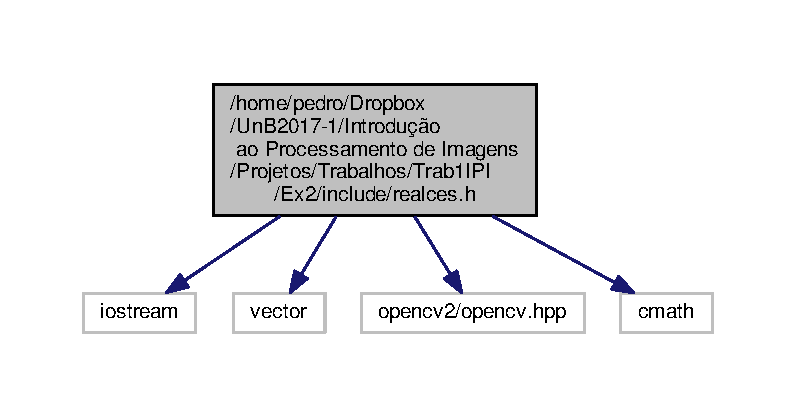
\includegraphics[width=350pt]{realces_8h__incl}
\end{center}
\end{figure}
This graph shows which files directly or indirectly include this file\+:
\nopagebreak
\begin{figure}[H]
\begin{center}
\leavevmode
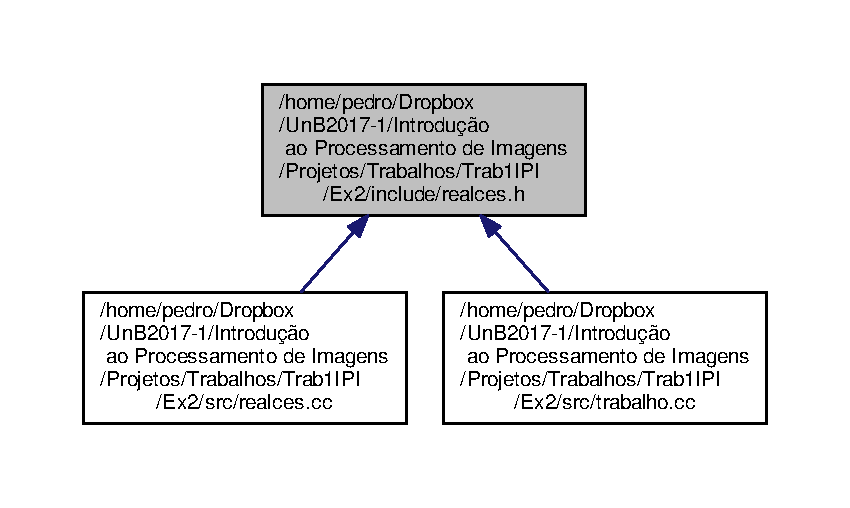
\includegraphics[width=350pt]{realces_8h__dep__incl}
\end{center}
\end{figure}
\subsection*{Functions}
\begin{DoxyCompactItemize}
\item 
Mat \hyperlink{realces_8h_a7ef97641d3e69f65f7d1acb790425d62}{trans\+\_\+power\+\_\+law} (char $\ast$img, double fator)
\begin{DoxyCompactList}\small\item\em Filtro de realce exponencial. \end{DoxyCompactList}\item 
Mat \hyperlink{realces_8h_a9ac8c44030210f21ddd39f2b9d69cea0}{trans\+\_\+hist} (char $\ast$img)
\begin{DoxyCompactList}\small\item\em Filtro de histograma. \end{DoxyCompactList}\end{DoxyCompactItemize}


\subsection{Detailed Description}
Arquivo que contém a biblioteca de \hyperlink{realces_8cc}{realces.\+cc}. 

\begin{DoxyAuthor}{Author}
Pedro Nogueira -\/ 14/0065032 
\end{DoxyAuthor}


\subsection{Function Documentation}
\index{realces.\+h@{realces.\+h}!trans\+\_\+hist@{trans\+\_\+hist}}
\index{trans\+\_\+hist@{trans\+\_\+hist}!realces.\+h@{realces.\+h}}
\subsubsection[{\texorpdfstring{trans\+\_\+hist(char $\ast$img)}{trans_hist(char *img)}}]{\setlength{\rightskip}{0pt plus 5cm}Mat trans\+\_\+hist (
\begin{DoxyParamCaption}
\item[{char $\ast$}]{img}
\end{DoxyParamCaption}
)}\hypertarget{realces_8h_a9ac8c44030210f21ddd39f2b9d69cea0}{}\label{realces_8h_a9ac8c44030210f21ddd39f2b9d69cea0}


Filtro de histograma. 

Aplicação do filtro de realce por histograma do constraste de imagens.


\begin{DoxyParams}{Parameters}
{\em img} & -\/ Imagem a ser filtrada \\
\hline
\end{DoxyParams}
\index{realces.\+h@{realces.\+h}!trans\+\_\+power\+\_\+law@{trans\+\_\+power\+\_\+law}}
\index{trans\+\_\+power\+\_\+law@{trans\+\_\+power\+\_\+law}!realces.\+h@{realces.\+h}}
\subsubsection[{\texorpdfstring{trans\+\_\+power\+\_\+law(char $\ast$img, double fator)}{trans_power_law(char *img, double fator)}}]{\setlength{\rightskip}{0pt plus 5cm}Mat trans\+\_\+power\+\_\+law (
\begin{DoxyParamCaption}
\item[{char $\ast$}]{img, }
\item[{double}]{fator}
\end{DoxyParamCaption}
)}\hypertarget{realces_8h_a7ef97641d3e69f65f7d1acb790425d62}{}\label{realces_8h_a7ef97641d3e69f65f7d1acb790425d62}


Filtro de realce exponencial. 

Aplicação do filtro de realce exponencial do constraste de imagens.


\begin{DoxyParams}{Parameters}
{\em img} & -\/ Imagem a ser filtrada \\
\hline
{\em fator} & -\/ Potência a ser usada no filtro \\
\hline
\end{DoxyParams}

\hypertarget{realces_8cc}{}\section{/home/pedro/\+Dropbox/\+Un\+B2017-\/1/\+Introdução ao Processamento de Imagens/\+Projetos/\+Trabalhos/\+Trab1\+I\+P\+I/\+Ex2/src/realces.cc File Reference}
\label{realces_8cc}\index{/home/pedro/\+Dropbox/\+Un\+B2017-\/1/\+Introdução ao Processamento de Imagens/\+Projetos/\+Trabalhos/\+Trab1\+I\+P\+I/\+Ex2/src/realces.\+cc@{/home/pedro/\+Dropbox/\+Un\+B2017-\/1/\+Introdução ao Processamento de Imagens/\+Projetos/\+Trabalhos/\+Trab1\+I\+P\+I/\+Ex2/src/realces.\+cc}}


Arquivo que contém os filtros de realce do contraste de imagens.  


{\ttfamily \#include $<$realces.\+h$>$}\\*
Include dependency graph for realces.\+cc\+:
\nopagebreak
\begin{figure}[H]
\begin{center}
\leavevmode
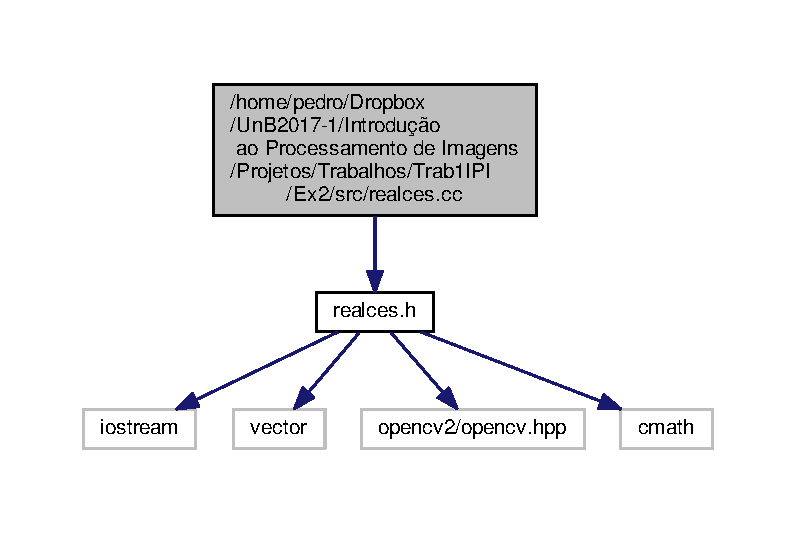
\includegraphics[width=350pt]{realces_8cc__incl}
\end{center}
\end{figure}
\subsection*{Functions}
\begin{DoxyCompactItemize}
\item 
Mat \hyperlink{realces_8cc_a7ef97641d3e69f65f7d1acb790425d62}{trans\+\_\+power\+\_\+law} (char $\ast$img, double fator)
\begin{DoxyCompactList}\small\item\em Filtro de realce exponencial. \end{DoxyCompactList}\item 
Mat \hyperlink{realces_8cc_a9ac8c44030210f21ddd39f2b9d69cea0}{trans\+\_\+hist} (char $\ast$img)
\begin{DoxyCompactList}\small\item\em Filtro de histograma. \end{DoxyCompactList}\end{DoxyCompactItemize}


\subsection{Detailed Description}
Arquivo que contém os filtros de realce do contraste de imagens. 

\begin{DoxyAuthor}{Author}
Pedro Nogueira -\/ 14/0065032 
\end{DoxyAuthor}


\subsection{Function Documentation}
\index{realces.\+cc@{realces.\+cc}!trans\+\_\+hist@{trans\+\_\+hist}}
\index{trans\+\_\+hist@{trans\+\_\+hist}!realces.\+cc@{realces.\+cc}}
\subsubsection[{\texorpdfstring{trans\+\_\+hist(char $\ast$img)}{trans_hist(char *img)}}]{\setlength{\rightskip}{0pt plus 5cm}Mat trans\+\_\+hist (
\begin{DoxyParamCaption}
\item[{char $\ast$}]{img}
\end{DoxyParamCaption}
)}\hypertarget{realces_8cc_a9ac8c44030210f21ddd39f2b9d69cea0}{}\label{realces_8cc_a9ac8c44030210f21ddd39f2b9d69cea0}


Filtro de histograma. 

Aplicação do filtro de realce por histograma do constraste de imagens.


\begin{DoxyParams}{Parameters}
{\em img} & -\/ Imagem a ser filtrada \\
\hline
\end{DoxyParams}
\index{realces.\+cc@{realces.\+cc}!trans\+\_\+power\+\_\+law@{trans\+\_\+power\+\_\+law}}
\index{trans\+\_\+power\+\_\+law@{trans\+\_\+power\+\_\+law}!realces.\+cc@{realces.\+cc}}
\subsubsection[{\texorpdfstring{trans\+\_\+power\+\_\+law(char $\ast$img, double fator)}{trans_power_law(char *img, double fator)}}]{\setlength{\rightskip}{0pt plus 5cm}Mat trans\+\_\+power\+\_\+law (
\begin{DoxyParamCaption}
\item[{char $\ast$}]{img, }
\item[{double}]{fator}
\end{DoxyParamCaption}
)}\hypertarget{realces_8cc_a7ef97641d3e69f65f7d1acb790425d62}{}\label{realces_8cc_a7ef97641d3e69f65f7d1acb790425d62}


Filtro de realce exponencial. 

Aplicação do filtro de realce exponencial do constraste de imagens.


\begin{DoxyParams}{Parameters}
{\em img} & -\/ Imagem a ser filtrada \\
\hline
{\em fator} & -\/ Potência a ser usada no filtro \\
\hline
\end{DoxyParams}

\hypertarget{trabalho_8cc}{}\section{/home/pedro/\+Dropbox/\+Un\+B2017-\/1/\+Introdução ao Processamento de Imagens/\+Projetos/\+Trabalhos/\+Trab1\+I\+P\+I/\+Ex1/src/trabalho.cc File Reference}
\label{trabalho_8cc}\index{/home/pedro/\+Dropbox/\+Un\+B2017-\/1/\+Introdução ao Processamento de Imagens/\+Projetos/\+Trabalhos/\+Trab1\+I\+P\+I/\+Ex1/src/trabalho.\+cc@{/home/pedro/\+Dropbox/\+Un\+B2017-\/1/\+Introdução ao Processamento de Imagens/\+Projetos/\+Trabalhos/\+Trab1\+I\+P\+I/\+Ex1/src/trabalho.\+cc}}


Arquivo do primeiro exercício do primeiro trabalho de I\+PI UnB -\/ 1/2017.  


{\ttfamily \#include $<$dec\+\_\+int.\+h$>$}\\*
{\ttfamily \#include $<$edge\+\_\+improv.\+h$>$}\\*
Include dependency graph for trabalho.\+cc\+:
\nopagebreak
\begin{figure}[H]
\begin{center}
\leavevmode
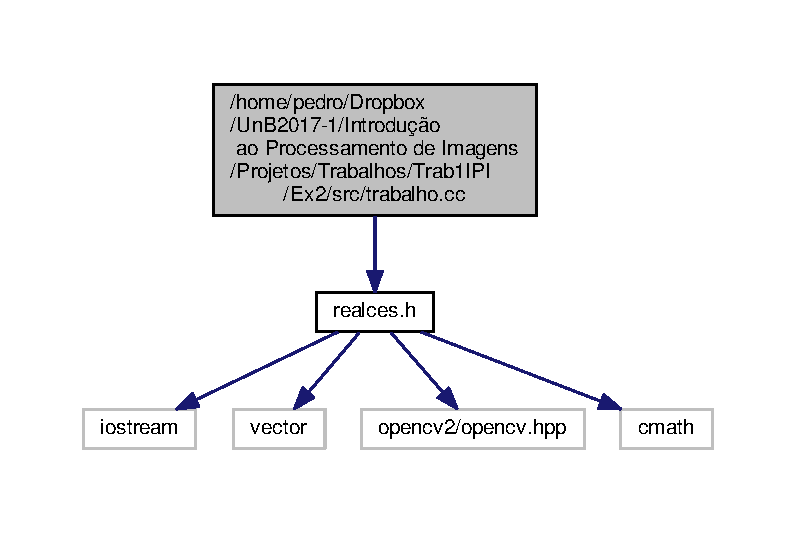
\includegraphics[width=261pt]{trabalho_8cc__incl}
\end{center}
\end{figure}
\subsection*{Functions}
\begin{DoxyCompactItemize}
\item 
int \hyperlink{trabalho_8cc_ae66f6b31b5ad750f1fe042a706a4e3d4}{main} ()
\begin{DoxyCompactList}\small\item\em Main do programa. \end{DoxyCompactList}\end{DoxyCompactItemize}


\subsection{Detailed Description}
Arquivo do primeiro exercício do primeiro trabalho de I\+PI UnB -\/ 1/2017. 

\begin{DoxyAuthor}{Author}
Pedro Nogueira -\/ 14/0065032 
\end{DoxyAuthor}


\subsection{Function Documentation}
\index{trabalho.\+cc@{trabalho.\+cc}!main@{main}}
\index{main@{main}!trabalho.\+cc@{trabalho.\+cc}}
\subsubsection[{\texorpdfstring{main()}{main()}}]{\setlength{\rightskip}{0pt plus 5cm}int main (
\begin{DoxyParamCaption}
{}
\end{DoxyParamCaption}
)}\hypertarget{trabalho_8cc_ae66f6b31b5ad750f1fe042a706a4e3d4}{}\label{trabalho_8cc_ae66f6b31b5ad750f1fe042a706a4e3d4}


Main do programa. 

Mostra imagens bonitinhas. 
%--- End generated contents ---

% Index
\backmatter
\newpage
\phantomsection
\clearemptydoublepage
\addcontentsline{toc}{chapter}{Index}
\printindex

\end{document}
